\section{Chip Layout}
    \subsection{PIN Layout}
        The layout for our 16x16 Programmable Interconnect Network is shown
        below.  The component on the bottom left are two 2:1 muxes which are
        used for test mode.
        \begin{figure}[H]
            \centering
            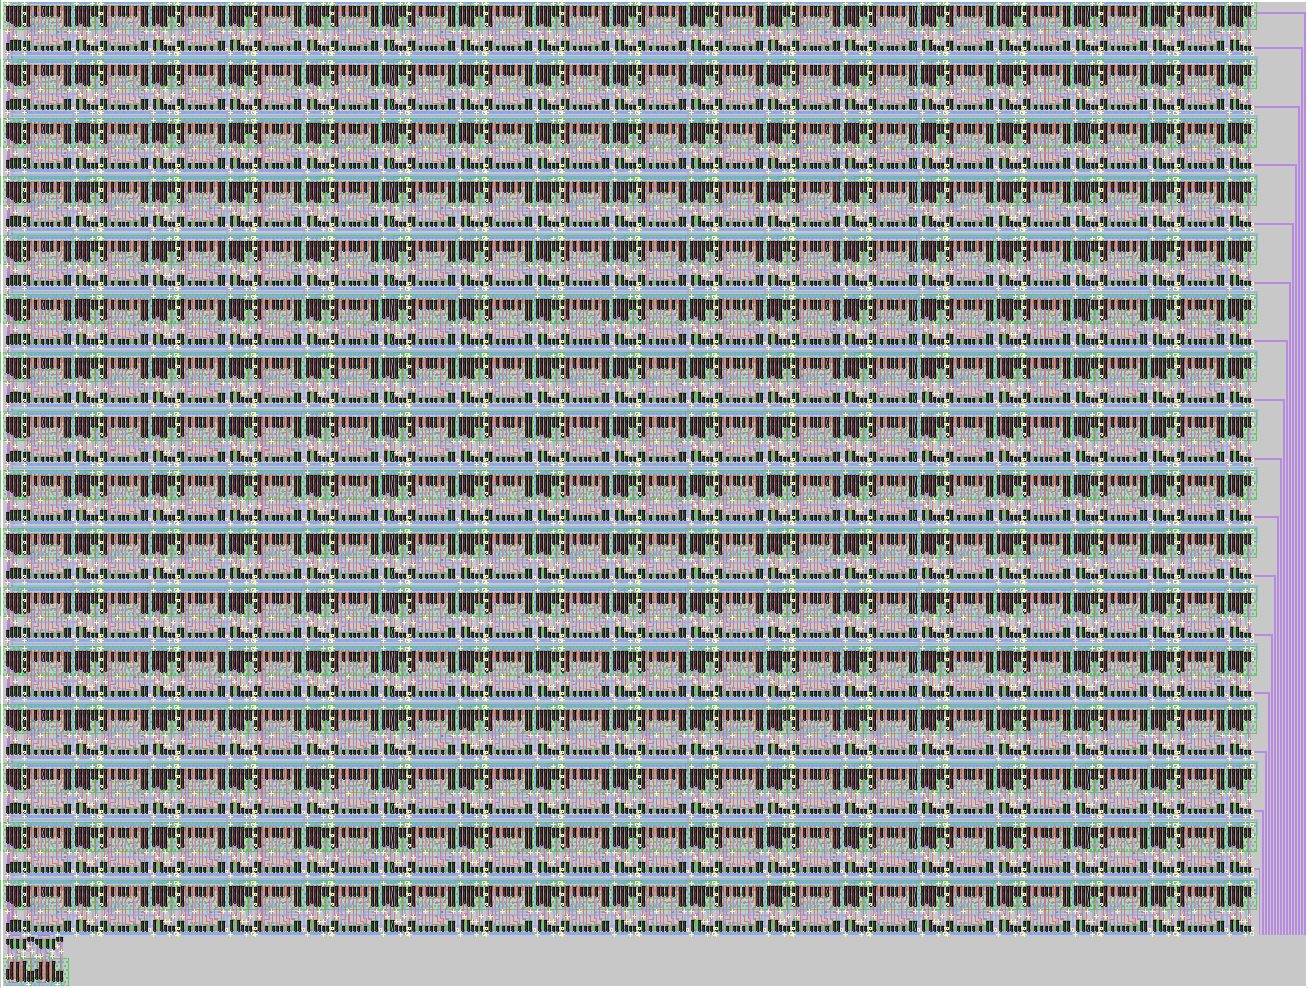
\includegraphics[width=\linewidth]{../../magic/images/pin.png}
            \caption{PIN Layout}
        \end{figure}
    \subsection{Shifter Layout}
        The layout for our 16 bit parallel-load parallel-output shifter
        register is shown below. At 16 bits the shifter just fits within the
        frame of our chip.  The component on the top right is a 2:1 mux which
        is used for test mode.
        \begin{figure}[H]
            \centering
            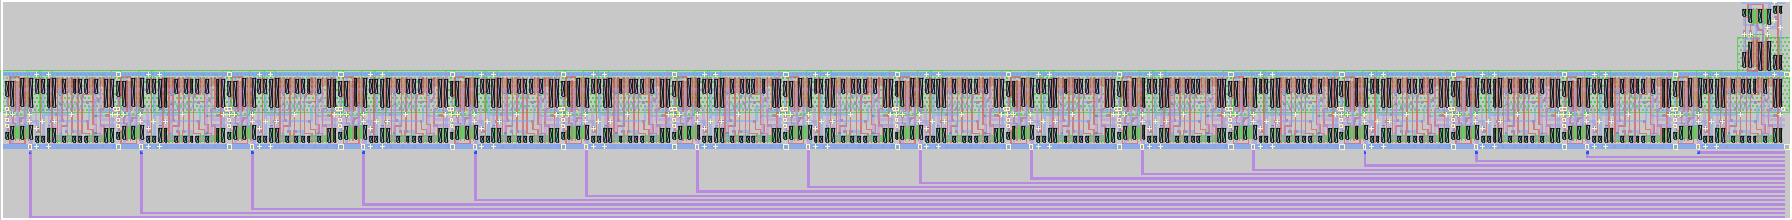
\includegraphics[width=\linewidth]{../../magic/images/shift.png}
            \caption{Shifter Layout}
        \end{figure}
    \subsection{Overall Layout}
        The final layout for Intranex is shown below. While our design spans
        the full width of the frame we had quite a bit of empty vertical space.
        We used this extra area to include a fun logo.
        \begin{figure}[H]
            \centering
            \includegraphics[width=\linewidth]{../../magic/images/intranex.png}
            \caption{Overall Layout}
        \end{figure}

        \newpage
        The same layout in its flattened form is shown below.
        \begin{figure}[H]
            \centering
            \includegraphics[width=\linewidth]{../../magic/images/intranex_flat.png}
            \caption{Overall Layout (Flattened)}
        \end{figure}

\newpage
\section{Users Guide}
The typical use case for Intranex is manipulating the order of bits in a
vector. As an example lets see how we can use Intrnex to flip the bit order of
a 16bit vector.

Lets choose 0b0111110000110001 as our input vector and its flipped form
0b1000110000111110 as our target result. In order to flip the vector we
will need to configure the PIN mapping as such:

\begin{verbatim}
0 0 0 0 0 0 0 0 0 0 0 0 0 0 0 1    0
0 0 0 0 0 0 0 0 0 0 0 0 0 0 1 0    1
0 0 0 0 0 0 0 0 0 0 0 0 0 1 0 0    2
0 0 0 0 0 0 0 0 0 0 0 0 1 0 0 0    3
0 0 0 0 0 0 0 0 0 0 0 1 0 0 0 0    4
0 0 0 0 0 0 0 0 0 0 1 0 0 0 0 0    5
0 0 0 0 0 0 0 0 0 1 0 0 0 0 0 0    6
0 0 0 0 0 0 0 0 1 0 0 0 0 0 0 0    7  <--- Output value bit position (hex)
0 0 0 0 0 0 0 1 0 0 0 0 0 0 0 0    8
0 0 0 0 0 0 1 0 0 0 0 0 0 0 0 0    9
0 0 0 0 0 1 0 0 0 0 0 0 0 0 0 0    A
0 0 0 0 1 0 0 0 0 0 0 0 0 0 0 0    B
0 0 0 1 0 0 0 0 0 0 0 0 0 0 0 0    C
0 0 1 0 0 0 0 0 0 0 0 0 0 0 0 0    D
0 1 0 0 0 0 0 0 0 0 0 0 0 0 0 0    E
1 0 0 0 0 0 0 0 0 0 0 0 0 0 0 0    F
-------------------------------
0 1 2 3 4 5 6 7 8 9 A B C D E F    <--- Input value bit posisition (hex)
\end{verbatim}

As we can see the value at input bit position 0 will end up at output bit
position 15 since that grid cell is marked as a 1, indicating a connection.

The PIN vector is shifted in on the \texttt{PSI} pin starting at the top-right
of the network. For our example the first 48 bits shifted in would be: (note we
are shifting the left-most bit in the following string first)

\begin{verbatim}
1000000000000000 0100000000000000 0010000000000000 ...
\end{verbatim}

The timing diagram below illustrates clocking in the first 20 and last 3 bits of our PIN configuration.

\begin{figure}[H]
    \centering
    \includegraphics[width=\linewidth]{../waveforms/example_pin.png}
    \caption{PIN Configuration Example}
\end{figure}

In order to clock in the input vector we simply use the \texttt{SCLKI} and
\texttt{SI} pins to clock the vector in most significant bit first. After the
input has been clocked in the \texttt{LDI} pin must be asserted and the
\texttt{SCLKI} line pulse to latch the result vector. The MSB of the result is
available immediately on \texttt{SO}. The remaining 15 bits of the result can
then be clocked out. A diagram illustrating this process for our example is
shown below.

\begin{figure}[H]
    \centering
    \includegraphics[width=\linewidth]{../waveforms/example_load_read.png}
    \caption{Loading the input vector and reading the result}
\end{figure}


\section{Test Strategy}

\subsection{Independent Logic Gates}
The are a few different strategies to go about testing our chip. The first
involves the independent gates and slices placed at the top of our chip.  The
\texttt{Test Inverter}, found on pins \texttt{3} and \texttt{4}, along with the
standard D-Flip Flop, found on pins \texttt{28-30}, can be used to ensure the
die is structurally valid and that power is being delivered on the distribution
rails.

\subsection{Independent Slices}
Secondly, there are two independent slices which can be used for verification.
On pins \texttt{31-35} there are connections to a single \texttt{Shift Slice}
which can be used to verify its operation. The expected operation of this slice
has been discussed heavily in previous sections of this document. There is also
an independent \texttt{PIN Slice} found on pins \texttt{37-40} and \texttt{1-2}.
Like this \texttt{Shift Slice}, this slice can be used to prove the functionality
of the design and layout.

\subsection{Test Mode}
To confirm that the main functional blocks are connected the \texttt{TESTI} pin
can be asserted which will enabled the design to function as a scan chain. With
\texttt{TESTI} asserted all 272 flip flops in the design are chained together.
Clocking a pulse into the \texttt{SI} pin using the \texttt{SCLKI} clock pin
should result in the same pulse appearing on the \texttt{SO} pin 272 clock
cycles later.

\subsection{Internal Signals}
The output of nine rows of the PIN are brought out onto dedicated debugging
pins \texttt{11-15} and \texttt{17-20}. These signals can be used to ensure
that the PIN is operating correctly and can be used to confirm that the
parallel load shifter is parallel loading the correct values.

\subsection{Function Test}
Finally, a standard functional test can be used with known vectors. For
instance, a good vector to test is one that reverses the bit order of the input
vector. This configuration is ideal as it allows for quick human validation.
An example of this has been shown in previous sections.

\newpage
\section{Chip Architecture}

As has been discussed the architecture of our chip is broken up into two major
parts: the Programmable Interconnect Network, and the Parallel-Load
Parallel-Output Shifter Register. Our design has remained fairly consistent
throughout our project with the only major change between progress reports
being a slight modification to our slices to squeeze out a few more lambdas.
This optimization ultimately lead us to achieve a PIN of 16x16 which we are
satisfied with as 16 is a nice clean number. With input vectors of 16 bits we
can now accomplish interesting tasks such as switching the endianess of words.

In order to handle the large fanout of the PIN clock we added buffers to the
beginning of each PIN row. Each buffer provides more than enough drive strength
to clock the entire row. Additionally, we opted to not include a buffer on the
shift register as the fanout is fairly low.

\newpage
\section{Simulation Results}

    \subsection{Test Mode}

    For the overall simulation of the final chip the first thing we tested was
    Test Mode.  A simple IRSIM CMD file was written, shown below, to send a
    pulse through and assert that it is received after 272 clock pulses, which
    is the number of flip-flops in our chain.

    \lstinputlisting[caption=Intranex Test Mode IRSIM CMD File, language=bash]{../../irsim/intranex_test.cmd}

    While the figure below provides little to no value it is included here for
    formality. The waveforms at this level are of little use to us since we are
    working with events that happen every couple hundred clocks.  This is why
    we chose to use the assertion feature of IRSIM to check the output.
    \begin{figure}[H]
        \centering
        \includegraphics[width=\linewidth]{../../irsim/intranex_test_mode.png}
        \caption{Intranex Test Mode IRSIM Result}
    \end{figure}

    \newpage
    \subsection{Functional Mode}
    For a functional test we configured the PIN to simply flip the input value.
    In the high level waveform shown below we can see the PIN being configured
    followed by the input value be shifted in and the result shifted out.
    \begin{figure}[H]
        \centering
        \includegraphics[width=\linewidth]{../../irsim/intranex.png}
        \caption{Intranex Functional Mode IRSIM Result}
    \end{figure}

    Taking a closer look at the input-output waveforms we can see that we clock
    in a value of \texttt{0111110000110001}. The \texttt{LDO} line, which is a
    passthrough from \texttt{LDI}, shows us that we then latched the result
    vector. The result vector is then shifted out and as we can see the
    expected output, \texttt{1000110000111110}, is achieved.
    \begin{figure}[H]
        \centering
        \includegraphics[width=\linewidth]{../../irsim/intranex_zoom.png}
        \caption{Intranex Functional Mode IRSIM Result (zoomed)}
    \end{figure}

    \newpage
    It would be impossible to exhaustively test our design at this scale so we
    settled for a random check over a few hundred input vectors. To achieve
    this a program was written to first generate a random input vector, a
    random permutation of the input vector, and the PIN configuration vector
    required to achieve the permutation. The program then writes the IRSIM
    \texttt{cmd} file for this setup which has assertions to check if the
    output is correct. Our program than launches IRSIM, which logs its output
    to a file, and then checks the resulting log for any assertion fails. If
    no assertion failed it continues to the next test. A screenshot showing the
    tester in action is shown below.

    \begin{figure}[H]
        \centering
        \includegraphics[width=\linewidth]{../../irsim/terminal.png}
        \caption{Automated Testing Screenshot}
    \end{figure}

    \newpage
    The source code for the automated tester is included below:

    \lstinputlisting[caption=Python Intranex Automated Tester, language=Python]{../../irsim/intranex.py}

    \newpage
    \subsection{Timing Analysis}

    In order to determine the worst case delay through our chip we used a
    modified version of the automated test program which generated an IRSIM
    command file for a single input vector and also included a \texttt{PATH}
    statement. The \texttt{PATH} statement, which we also used to time the
    slices in Part 2, shows us the worst case delays for every input state
    change. After running our program we have an IRSIM log with the delays for
    each of the 16 state changes. The delays are unfortunately presented per net
    and are not automatically totalled. A small program, \texttt{find\_delay.py},
    was written to parse the log and add up the net delays for each input vector.
    It then returns the longest delay time. Doing this over various vectors we
    found our worst case delay to be consistently around \textbf{2.51ns}. This
    indicates a max clock speed of \textbf{398MHz}.

    An example showing the analysis flow is shown below:
    \begin{lstlisting}[language=bash]
    $ python intranex_single.py \
    0001000000000000\
    0000000000000010\
    { 12 lines snipped }
    0000001000000000\
    0000000001000000 1010000011110001 1000011010011100
    $ python find_delay.py intranex.log
    Worst delay: 2.510000
    \end{lstlisting}

    The source code for the delay parser is shown below:
    \lstinputlisting[caption=Delay Parser, language=Python]{../../irsim/find_delay.py}

    \section{Work Division}

        \begin{table}[H]
            \centering
            \begin{tabular}{ll}
                \toprule
                \textbf{Task} & \textbf{Person}\\
                \midrule
                PIN Layout            & Thrun \\
                Shift Layout          & Qi \\
                Overall Layout        & Thrun \\
                Users Guide           & Qi \\
                Testing Strategy      & Qi \\
                Chip Architecture     & Thrun \\
                Simulation Test Mode  & Thrun \\
                Simulation Functional & Both \\
                Simulation Timing     & Qi \\
                \bottomrule
            \end{tabular}
            \caption{Task Assignment}
        \end{table}

